% Paper 2 — full ICLR 2027 submission (expanded from the workshop-length p2_tools.tex).
% NOTE: uses the vendored ICLR 2026 style as a stand-in; the ICLR 2027 template
% (github.com/ICLR/Master-Template/raw/master/iclr2027.zip) was not yet posted at
% time of writing. Swap the two style lines for iclr2027_conference when it releases
% (near-identical year to year). Double-blind; anonymous. 9-page limit (refs/appendix free).
\documentclass{article}
\usepackage{iclr2026_conference,times}
\usepackage{natbib}
\usepackage{amsmath,amssymb}
\usepackage{booktabs}
\usepackage{xcolor}
\usepackage{hyperref}
\usepackage{microtype}
\usepackage{graphicx}
\newcommand{\pending}[1]{\textcolor{orange!80!black}{[#1]}}
\newcommand{\kap}{\kappa}

\title{Which Bias Flags Can You Trust?\\
A Label-Free Triage Protocol for\\
Frontier-Model News-Bias Detection}
\author{Anonymous Authors\\
\texttt{anonymous@example.com}}

\begin{document}
\maketitle

\begin{abstract}
News-bias products---bias checkers, balanced-news feeds, media-literacy
tools---are increasingly built by asking a frontier model to flag biased
spans, label an article's lean, and explain itself. Which of those
outputs can a builder trust, and how should the untrustworthy ones be
triaged \emph{without} ground-truth labels at inference time? Evaluating
two frontier target models and two cross-family judges on 200 U.S.\
news articles carrying outlet-anchored AllSides ratings, we first map the primitives: the
\emph{volume} of flagged spans is a valid partisan-intensity meter
(Spearman $\rho \approx 0.6$), and models rank-track the continuous
expert lean rating at $\rho \approx 0.8$, but a single model's lean
label near the center-right, its omission and unsupported-claim flags
(chance-corrected agreement $\kap \le 0.15$), and the specific text it highlights
(cross-model overlap $0.26$) are model-specific opinion. We then turn the
map into a validated selective-prediction protocol. A label-free
\emph{committee-disagreement} bit (one extra model call, no annotation)
is not distinguishable from a calibrated confidence score as an error
ranker at this sample size (AUC $0.70$ vs $0.74$), shows a directional
(non-significant) error-capture advantage at $20$--$30\%$ review
budgets ($+6$--$7$pts; committee picks are $34\%$ accurate on
disagreements vs $74\%$ on agreements, part of the gap structural), and
combined with confidence yields the lowest risk--coverage area of any
signal (AURC $0.20$ vs $0.21$ confidence, $0.31$ disagreement); a
two-vendor four-model unanimity gate clears $44\%$ of articles at
$87\%$ accuracy; and neither raw confidence (both models overconfident; a stated
$0.9$ means ${\sim}75\%$) nor a majority-vote ensemble (no accuracy gain
over the best single model) should be used as a probability. The two headline results hold across five prompt conditions, and the
reliability map and the directional failure both replicate on a six-model committee spanning
four independent labs (Anthropic, OpenAI, Alibaba, DeepSeek). Findings
are exploratory and inherit AllSides outlet labels as ground truth;
headline statistics carry article-level bootstrap CIs (committed
scripts reproduce every number).
\end{abstract}

\section{Introduction}
A growing class of products puts a frontier language model in the role
of a news-bias analyst: it highlights loaded spans, assigns a
left/right lean, summarizes ``both sides,'' and narrates why. The
implicit assumption is that these outputs are measurements. Many are
not---they are one model's opinion, and a different frontier model,
shown the same article, would say something else. A builder needs two
things before shipping: to know \emph{which} outputs reproduce, and---for
the ones that do not---a way to catch the likely errors that needs
\emph{no} ground-truth labels at inference time, since a deployed
product has none.

This paper supplies both. We do not ask whether the models are biased (a
companion study takes up the behavioral question); we ask which of a
bias detector's outputs a tool can present as reliable, and how to
triage the rest. Our answer is a reliability map with a clean split---
primitives anchored to explicit text reproduce across independent
models; primitives that require inference about what is absent or
implied do not---and, built on it, a label-free triage protocol whose
central signal is not model confidence but \emph{model disagreement}. We
validate the protocol against the standard confidence baseline with a
risk--coverage operating curve, and show it is stable across prompt
conditions and across four independent model vendors rather than an
artifact of one.

\textbf{Contributions.}
\begin{enumerate}
  \item \textbf{A reliability map of bias-detection primitives.} Which
  outputs of a frontier-model bias detector reproduce across models
  (detection volume; continuous-rating rank; cross-model agreement) and
  which are model-specific opinion (lean labels near center-right;
  omission and unsupported-claim flags; specific highlights)---each with a number
  and a bootstrap CI (\S\ref{sec:map}).
  \item \textbf{A validated, label-free triage protocol.} A label-free
  committee-disagreement router with a published risk--coverage operating
  curve, benchmarked against a calibrated confidence router (not
  distinguishable as an error ranker at this $n$; a directional
  in-budget capture advantage; lowest AURC when combined); a high-precision unanimity
  gate; and a per-model calibration analysis showing raw confidence must
  be rescaled and is trustworthy only for direction (\S\ref{sec:triage}).
  \item \textbf{A directional failure mode shared across four vendors.}
  All six models we evaluate---across four independent labs---read
  moderate-right content as center-or-left, so a lean-labeling tool built
  on them under-counts the right; stable across five prompt conditions
  (\S\ref{sec:fail}).
\end{enumerate}

\section{Related Work}
\textbf{LLM-as-judge reliability.} Using an LLM to score model outputs is
now standard \citep{zheng2023judging}, and its biases---position,
verbosity, self-preference---are documented
\citep{ye2024justice,panickssery2024selfpreference}. Reliability with
consequences is emerging at the \emph{instance} level (selective
evaluation with human-agreement guarantees and escalation
\citep{jung2025trust}) and judge \emph{selection} by human agreement is
practiced in benchmark construction \citep{dubois2024length,lambert2024tulu}.
We differ in object and use: rather than validating a judge for
scoring, we ask which \emph{primitives} of a frontier bias detector a
downstream product can trust, and we supply a deployment-time triage
signal that needs no human labels at all.

\textbf{Selective prediction.} Deferring uncertain cases to a human is
classical selective classification, evaluated by the risk--coverage curve
\citep{elyaniv2010foundations,geifman2017selective}. Committee disagreement as an
error signal descends from query-by-committee \citep{seung1992query},
ensemble uncertainty \citep{lakshminarayanan2017simple}, and
disagreement-predicts-error results \citep{jiang2022assessing}; in the
LLM era, sampled self-consistency flags errors label-free
\citep{manakul2023selfcheckgpt} and diverse-model panels replace single
judges \citep{verga2024replacing};
our contribution is an operating-regime characterization for
frontier-model lean classification: the annotation-free disagreement bit
is not distinguishable from calibrated confidence as an error ranker at
our sample size, shows a directional capture advantage below the
disagreement rate, and combining the two signals yields the lowest
risk--coverage area---measured head-to-head with article-clustered
uncertainty throughout.

\textbf{Political bias in LLMs, and news tasks.} A large literature
measures LLM political orientation, largely via questionnaires
\citep{feng2023pretraining,santurkar2023opinions}, whose validity as a
behavioral measure is contested \citep{rottger2024political}. Closer to
our task, concurrent work reports ``ideological center-collapse'' in
frontier-model news classification and steered generation on
AllSides-labeled articles \citep{kennedy2026left}. We are not measuring
bias but the \emph{reliability} of a bias detector's outputs; where we do
report a directional error (\S\ref{sec:fail}), our per-class
decomposition refines the center-collapse observation into a
right-to-left asymmetry and replicates it across four labs.

\textbf{Bias detection in NLP.} Span-level media-bias detection is an
established task \citep{spinde2021babe,hamborg2019automated} using
outlet-anchored corpora such as AllSides \citep{baly2020detect}; we adopt
that lineage and ground truth and study what a frontier model's outputs
on it can and cannot support.

\section{Setup}
\label{sec:setup}
We reuse the corpus, models, and rollouts of the companion study; we
summarize here and defer the full protocol (including the pre-committed
reliability gates behind the judge instruments) to it. The corpus is
$N{=}200$ contemporary U.S.\ news articles on a balanced $5\times8$
grid: five AllSides-anchored lean classes (Left, Lean~Left, Center,
Lean~Right, Right; 40 each) crossed with eight topics, 400--1500 words,
each also carrying a continuous expert lean rating. Models receive
\emph{article text only}---no outlet, headline, URL, or date---so
classification cannot reduce to outlet priors.

Two frontier \emph{target} models (Claude Sonnet~4.5, GPT-4.1) and two
cross-family \emph{judge} models (Claude Sonnet~4.6, GPT-5) perform three
tasks: span-level bias detection with a shared bias-type schema
\citep{spinde2021babe,hamborg2019automated}, summarization with
represented-perspective counts, and five-class lean classification with a
self-reported confidence. Two further open-weight judges
(Qwen3-235B-A22B, Alibaba; DeepSeek-V3.2), added post hoc via
HuggingFace Inference Providers, extend the classification committee to
six models across four labs for the four-family checks
(\texttt{analysis/rate\_articles\_ext.py}). All analyses are exploratory
(not pre-registered) and use expert AllSides labels as ground truth
\citep{baly2020detect}; agreement is Cohen's $\kap$, and bootstrap CIs
use $10^4$ resamples with a fixed seed. Data accounting: $N{=}200$ v3 articles; router
analyses use the $199$ with both targets parsed (baseline); the
six-model checks the $198$ rated by all six; legacy pilot rollouts
sharing these directories are excluded throughout
(\texttt{results/rollout/LEGACY\_NOTE.md}).

\section{Which primitives reproduce}
\label{sec:map}

\textbf{Detection volume is a valid intensity meter.} The simplest
signal---how many spans a model flags---tracks how loaded an article is:
flagged-span count rises monotonically with the article's expert-rated
intensity (Spearman $\rho{=}0.64$ Sonnet, $0.58$ GPT-4.1 against
$|\text{lean rating}|$, both $p{<}10^{-18}$; partisan articles draw
$2.3\times$ the flags of Center articles). A builder can trust a flag
\emph{count} as a meter even where the individual flags are unreliable.

\textbf{Lean predictions track the continuous rating, not just the
bucket.} Each model's five-class prediction rank-correlates with the
\emph{continuous} expert rating at least as strongly as with the discrete
label (Spearman $0.77$--$0.86$ across the four models; difference vs the
label $\le 0.01$), and within a single label class the models resolve
graded intensity the bucket discards (within-Lean-Left
$\rho(\text{pred},\text{rating}){=}0.40$--$0.50$, $p\le.01$, all four).
The lean signal is thus finer than the five-way label, and the results
below are not an artifact of five-way bucketing. (We do not claim
independence from the AllSides labels: the continuous rating and the
discrete label partition this corpus identically.)

\textbf{Only concrete, word-anchored bias forms reproduce.} Given both
target models the same bias-type schema, we measure how often they agree
a form is present (Cohen's $\kap$ over the 200 jointly-rated v3
articles, Table~\ref{tab:biastype}). Agreement spans $0.53$ down to
$0.08$: the word-anchored forms reach moderate agreement
(opinion-stated-as-fact $0.53$, subjective adjectives $0.47$)---and the forms defined by what
is \emph{absent from} or \emph{unverified against} the text collapse
toward chance. The disagreement is not random: the two models have
distinct habits---Claude leads with bias-by-omission ($14\%$ of its
flags), GPT-4.1 with sensationalism ($15\%$)---so one hunts what a story
omits while the other hunts its tone, which is exactly why they cannot
agree omission is present. The unreliability reaches the span level:
even when both flag the same article, the specific highlighted text
overlaps at only Jaccard $0.26$. For a tool: show concrete word-level
flags; treat any single model's omission, framing, or unsupported-claim
flag---and any individual highlight---as one model's opinion, surfaced
only on cross-model agreement.

\begin{table}[t]\centering\small
\begin{tabular}{lc@{\hskip 2em}lc}
\toprule
Reliably agreed ($\kap$) & & Barely above chance ($\kap$) & \\
\midrule
opinion stated as fact & $0.53$ & omission of attribution & $0.23$ \\
subjective adjectives & $0.47$ & story choice \& placement & $0.20$ \\
mind reading & $0.43$ & bias by omission & $0.15$ \\
word choice & $0.38$ & unsubstantiated claims & $0.08$ \\
\bottomrule
\end{tabular}
\caption{Cross-model agreement on bias forms (Cohen's $\kap$, two target
models, 200 shared v3 articles). Detectability tracks textual explicitness:
models agree on loaded \emph{words}, not on what a story \emph{left out}
or whether a claim is \emph{unsupported}.}
\label{tab:biastype}
\end{table}

\textbf{A cheap word-list is a corpus monitor, not a per-item detector.}
A deterministic paired left/right lexicon corroborates aggregate
directional patterns, but as a filter for a judge's per-output verdict
it reaches only precision $0.25$, recall $0.30$---so it belongs in a
corpus-level regression check, never as a live per-article flag.

\section{A label-free triage protocol}
\label{sec:triage}
The map says most single-model outputs cannot be shown as fact. A
deployed product cannot fix this with ground truth---it has none at
inference---so it needs a trust signal computable from the model outputs
alone. We show the best such signal is \emph{model disagreement}, and
benchmark it against the obvious alternative, model confidence.

\textbf{Route disagreement first.} On five-class lean
($n{=}199$ articles, both targets parsed; committee pick on a
disagreement = the higher-confidence model's label), when the two
target models agree they are $73.8\%$ accurate ($n{=}122$); on
disagreements the committee pick is $33.8\%$ accurate ($n{=}77$; gap
$40.0$pts, article-clustered $95\%$ CI $[26.9, 53.3]$ --- noting a
structural component: on a disagreement at most one of the two labels
can be correct). As an error ranker the label-free disagreement bit is
not distinguishable from calibrated confidence at this sample size
(AUC $0.695$ vs $0.740$), and it shows a \emph{directional},
non-significant capture advantage in the operational regime
(Figure~\ref{fig:rc}, Table~\ref{tab:router}): at a $20$--$30\%$ review budget it captures
$+6$ to $+7$ points more of all errors than a confidence threshold
(clustered $p{=}.10$ and $p{=}.22$; pooling all five prompt conditions
does not reach significance either). Integrated over
\emph{all} coverage levels the picture is complementary: confidence,
being continuous, resolves risk within the agree and disagree groups and
so has a modestly lower area under the risk--coverage curve
(tie-robust expected AURC $0.217$ vs disagreement's $0.296$; random
$0.39$, oracle $0.102$), even though the two are tied on error ranking. The two signals
carry the same information but deliver it differently---disagreement is
\emph{free} and most powerful in the low-budget regime, confidence is
smoother across the curve---and \emph{combining} them (route
disagreements first, break ties within each group by confidence)
achieves the lowest area of any signal (AURC $0.201$), an ordering stable across all five
prompt conditions (disagreement AURC $0.29$--$0.34$, confidence
$0.19$--$0.22$, combined lowest or tied-lowest in every condition;
agree-vs-disagree accuracy $0.68$--$0.74$ vs $0.31$--$0.44$). The operational recommendation: \emph{route model
disagreements to human review first, rank within groups by confidence,
and expect no ranking gain from confidence alone until the budget exceeds
the disagreement rate.}

\begin{figure}[t]\centering
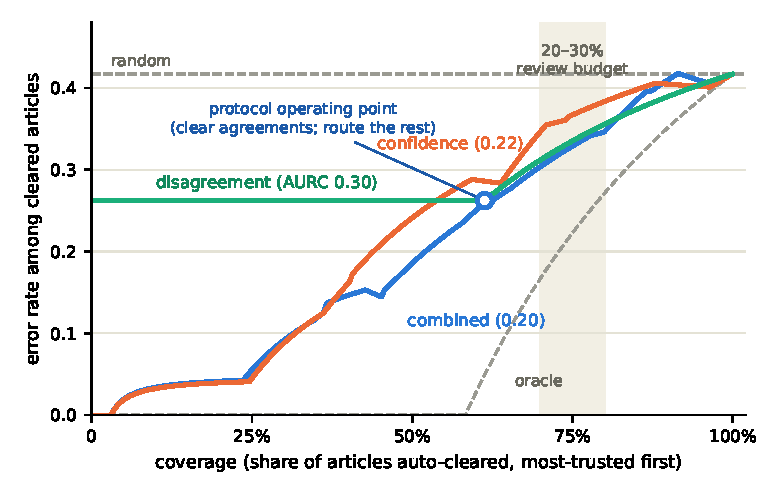
\includegraphics[width=0.82\linewidth]{figures/fig_risk_coverage}
\caption{Risk--coverage operating curves for the three routing signals
(baseline condition, $n{=}199$ articles; tie-robust expected risk, so
the binary disagreement signal is flat within its trust groups). Gray
dashed lines are the analytic random baseline and the oracle bound; the
shaded band is the practical $20$--$30\%$ review-budget regime.
Combining disagreement with confidence attains the lowest area (AURC in
parentheses). Reproduced by \texttt{analysis/fig\_risk\_coverage.py}.}
\label{fig:rc}
\end{figure}

\begin{table}[t]\centering\small
\begin{tabular}{lccccc}
\toprule
Review budget & $10\%$ & $20\%$ & $30\%$ & $40\%$ & $50\%$ \\
\midrule
route by disagreement & $10.8$ & $33.7$ & $48.2$ & $65.1$ & $78.3$ \\
route by confidence & $14.5$ & $26.5$ & $42.2$ & $59.0$ & $71.1$ \\
\bottomrule
\end{tabular}
\caption{Percent of all classification errors captured at each
human-review budget (route least-reliable first; $n{=}199$ v3 articles, two target
models). Disagreement leads confidence in the $20$--$50\%$ regime;
the advantage is directional (clustered $p{\ge}.10$).}
\label{tab:router}
\end{table}

\textbf{At committee scale, trust unanimity---not a vote.} Adding the two
judges, a four-model majority vote does \emph{not} beat the best single
model ($0.646$ vs $0.662$ exact; McNemar $p{=}.68$; bootstrap gain $95\%$
CI $[-.061,+.030]$), and a builder cannot pre-select which model will be
best (bootstrap $P(\text{is best})$: GPT-4.1 $.63$, Sonnet~4.6 $.35$,
GPT-5 $.02$, Sonnet~4.5 $.00$). Ensembling therefore buys robustness, not
accuracy. Its deployable value is instead a high-precision \emph{gate}:
the four models agree unanimously on $44\%$ of articles, and there they
are $87\%$ accurate---so unanimity auto-clears nearly half the volume at
high precision, and the residual is exactly the disagreement set the
router sends to review. A natural worry is that a committee-blind gate
would silently pass the shared directional failure of
\S\ref{sec:fail}; empirically it does not concentrate there --- the
true classes of the two-vendor gate's $11$ unanimous errors are spread
across Lean-Left ($4$), Center ($3$), and Lean-Right ($4$), and the
four-lab six-model gate clears $35\%$ of articles at $90\%$ accuracy
with only $2$ of its $7$ errors on Lean-Right
(\texttt{analysis/phase2\_analyses.py}).

\textbf{Never read raw confidence as a probability.} Consistent with
documented verbalized-confidence behavior
\citep{tian2023just,xiong2024can}, both models are
severely overconfident on the exact five-class label (mean confidence
$0.87$--$0.90$ vs accuracy $0.54$--$0.66$); a stated $0.9$ empirically
means $71\%$ (Claude) to $77\%$ (GPT-4.1) exact accuracy. GPT-4.1's
confidence is the better gate (Brier $0.259$ vs $0.333$; ECE $0.238$ vs
$0.330$), and---critically---
the overconfidence is almost entirely an \emph{exact-boundary} effect:
scored on lean \emph{direction} (within one class), GPT-4.1's confidence
is essentially calibrated (ECE $0.024$) and Claude's nearly so ($0.085$).
Confidence is a usable ordering for \emph{direction}, never a usable
probability for the exact label---rescale before thresholding.

\section{The directional failure mode}
\label{sec:fail}
The reproducible signals above are politically even-handed on average;
the classification \emph{errors} are not. Breaking accuracy down by true
class exposes a single hard case shared by every model
(Table~\ref{tab:byclass}): \emph{Lean~Right} is the hardest label for
every model we evaluate---all six, spanning four independent labs (exact
accuracy $0.07$--$0.46$), and difficulty falls as an article's expert
lean strengthens (Spearman $\rho{=}-0.37$, $p{<}10^{-7}$)---the models
read the poles well and lose the moderate right. The misreads are
\emph{directional}: misclassified Lean-Right articles are pulled
\emph{left}, not merely blurred to center---$33\%$ are labeled Lean-Left
or Left and $21\%$ Center, while Center articles are called Lean-Left
$32\%$ of the time versus Lean-Right $4\%$. A ``balanced feed'' or
lean-labeling product built on these classifications therefore
\emph{systematically under-counts right-leaning content}, consistent with
concurrent reports of ``center-collapse'' \citep{kennedy2026left}, which
our per-class decomposition refines into a right-to-left asymmetry.

\begin{table}[t]\centering\small
\begin{tabular}{lccccc}
\toprule
Model & Left & Lean~L & Center & \textbf{Lean~R} & Right \\
\midrule
Claude Sonnet 4.5 & $.97$ & $.23$ & $.50$ & $\mathbf{.07}$ & $.90$ \\
GPT-4.1 & $.88$ & $.47$ & $.75$ & $\mathbf{.46}$ & $.72$ \\
Claude Sonnet 4.6 & $.92$ & $.78$ & $.55$ & $\mathbf{.20}$ & $.80$ \\
GPT-5 & $.82$ & $.70$ & $.53$ & $\mathbf{.42}$ & $.60$ \\
Qwen3-235B & $.70$ & $.62$ & $.65$ & $\mathbf{.35}$ & $.72$ \\
DeepSeek-V3.2 & $.85$ & $.45$ & $.65$ & $\mathbf{.35}$ & $.68$ \\
\bottomrule
\end{tabular}
\caption{Exact classification accuracy by true lean class, six models
across four labs (targets: Claude Sonnet~4.5, GPT-4.1; judges: Claude
Sonnet~4.6, GPT-5, Qwen3-235B-A22B, DeepSeek-V3.2). Lean~Right is the
hardest label for every one. The bottom two rows are an exploratory
four-family extension via HuggingFace Inference Providers
(\texttt{analysis/rate\_articles\_ext.py}).}
\label{tab:byclass}
\end{table}

\textbf{The map holds across four independent labs.} Adding two
open-weight judges from two further families---Qwen3-235B-A22B (Alibaba)
and DeepSeek-V3.2 (DeepSeek)---extends the committee to six models over
four labs ($n{=}198$ articles rated by all six;
\texttt{analysis/four\_family\_analysis.py}). Every headline replicates.
Lean~Right is the hardest class for all six (Table~\ref{tab:byclass});
the agreement$\to$accuracy signal holds on all fifteen model pairs,
including the new cross-vendor ones (Qwen$\times$DeepSeek agree $0.69$ vs
disagree $0.45$; GPT-5$\times$DeepSeek $0.75$ vs $0.42$); consensus stays
a monotone accuracy signal, with six-model unanimity ($35\%$ of articles)
at $90\%$ accuracy; and the right-to-left misread is unchanged ($34\%$ of
Lean-Right articles labeled Lean-Left or Left, pooled across the six).
Replication across Anthropic, OpenAI, Alibaba, and DeepSeek rules out a
single-vendor quirk; it cannot, however, discriminate a shared
model-side bias from an artifact of the shared outlet-anchored labels
(all six models are scored against the same labels, and shared training
corpora are a common cause) --- only independent article-level labels
can separate these.

\textbf{Both the map and the failure are prompt-invariant.} Re-running
the two headline results under five different prompt scaffolds, the
agreement$\to$accuracy gap holds in all five (gap $0.28$--$0.36$,
bootstrap $P(\text{gap}{>}0){=}1.0$ in every condition) and Lean~Right is
the strict hardest class in all five (pooled accuracy $0.21$--$0.29$).
The pattern is a property of the models, not of one prompt. Nor is it
a class-boundary artifact: restricting Lean-Right articles to the core
band of their continuous rating (middle two quartiles) leaves the hole
unchanged (Sonnet $0.086$ vs $0.075$ on all; GPT-4.1 $0.412$ vs
$0.462$). Three riders. First, the Lean-Right effect is Claude-driven
(Claude is the worst model on it in $5/5$ conditions, GPT-4.1 in only
$3/5$). Second, the target contrast is not a simple quality ordering
but an \emph{engagement profile}: on clearly partisan articles (true
Left or Right, $n{=}80$ paired) Claude Sonnet~4.5 is significantly the
stronger reader ($0.94$ vs GPT-4.1's $0.80$; of the $13$ articles
exactly one model read correctly, Claude was right in $12$, McNemar
exact $p{=}.003$), and it produces the more substantive rationales
($175$ vs $94$ words on average) --- the same engagement that costs it
most in the subtle middle, where GPT-4.1's comparative reticence
protects it (post-hoc contrast;
\texttt{analysis/phase2\_analyses.py}). Third, lean classification is
least reliable on policy-abstract topics (elections/economy/climate) and
most reliable on identity-concrete ones.

\section{Discussion}
The results reduce to a short deployment policy for a news-bias product.
(1) \emph{Show decisions, filter prose, and rank flags by kind}: flag
counts and word-anchored flags are trustworthy; omission/framing/
unsupported-claim flags and individual highlights are one model's opinion
and should surface only on cross-model agreement. (2) \emph{Triage by
agreement, not raw confidence}: model disagreement is a free,
label-free error signal that beats a confidence threshold in the
realistic low-budget regime; combine the two for the best risk--coverage
trade-off, and never expose raw confidence as a probability. (3)
\emph{Correct for the rightward blind spot}: expect moderate-right
content to be under-labeled, and treat a ``center'' label on
right-of-center content as a routing trigger, not a verdict. None of
these require labels at inference; the only ground truth the protocol
needs is at build time, to choose thresholds. This turns a measurement
report into a reusable engineering recipe, and the corpus recipe and
analysis code are released so the map can be re-derived on a new model
generation cheaply.

\section{Limitations}
Three limits bound the claims. First, all findings are \emph{exploratory}
(not pre-registered) and inherit AllSides' outlet-anchored labels as the
sole ground truth \citep{baly2020detect}; the directional error could
partly reflect article-vs-outlet label drift, though uniform label noise
cannot produce a one-sided right-to-left pattern, and its replication
across four independent labs makes a pure-label explanation less likely.
A second, independent label source (per-article human consensus, or a
second rating provider) is the highest-value next test. Second, the
triage router is validated on the baseline prompt condition and one model
pair (though the reliability map and directional failure replicate across
conditions and vendors); and the label-free signals so far require a
\emph{committee}---disagreement needs two models, the unanimity gate four.
A single-model cold-start signal---SelfCheckGPT-style self-consistency
across temperature-sampled generations
\citep{manakul2023selfcheckgpt}, benchmarked against the disagreement
router's AUC of $0.70$---is a natural next step. Third, any LLM judge
inside a tool's own quality-control pipeline inherits the reliability
problem we document for the models themselves.

\section*{Ethics Statement}
This paper documents a directional reliability failure --- frontier
models under-label moderate-right news --- in politically sensitive
tooling, and we state its use explicitly: our evidence supports
\emph{escalating} affected items to human review, never automated or
editorial re-weighting of content by political direction; citing this
work as license to boost content of any lean misreads it. The ground
truth itself is contested --- outlet-anchored ratings projected to
articles --- and the failure is measured against, not independent of,
that standard. The reliability map is dual-use (it also tells an actor
which detector outputs are unauditable); we judge the builder and
auditor benefit to outweigh this, and release evaluation code rather
than any deployed classifier. News text is used under research norms
with article text redistributed only as required for reproduction.

\section*{Reproducibility Statement}
The corpus curation script and manifest, all task and judge prompts, the
runner, the four-family judging scripts
(\texttt{analysis/rate\_articles\_ext.py},
\texttt{analysis/four\_family\_analysis.py}), and per-call cost
accounting are released; every number in the paper is reproduced by these
scripts on the released rollouts. Bootstrap procedures use a fixed seed.
Article text is redistributed only as required for reproduction, with
source URLs and the deterministic curation script provided in lieu of
bulk redistribution where licensing requires. \pending{Repository and
data links after de-anonymization.}

\bibliography{references}
\bibliographystyle{iclr2026_conference}

\appendix
\section{Full four-family consensus ladder}
On the $n{=}198$ articles rated by all six models (four labs), modal-label
accuracy rises monotonically with the number of models agreeing:
$\ge2/6$ agree covers $100\%$ of articles at $0.66$; $\ge3/6$, $97\%$ at
$0.67$; $\ge4/6$, $81\%$ at $0.73$; $\ge5/6$, $48\%$ at $0.82$; $6/6$
(unanimous), $35\%$ at $0.90$. Unanimity across four independent vendors
is the strongest label-free confidence signal available.

\end{document}
